\documentclass[b5paper]{article}
% Add "final" option in the article to remove todo
\usepackage[tight,common_math_textnormal,todonotes,math_base_note,math_simple]{gatmeo}
\usepackage{tikz-cd}

\title{\bf{
Hypertoric Varieties Arose from Graphs
}}

\newcommand{\noskipline}{\vspace{-1.5em}}

\renewcommand{\epsilon}{\varepsilon}
\renewcommand{\phi}{\varphi}
\newcommand{\NN}{\mathbb{N}}
\newcommand{\ZZ}{\mathbb{Z}}
\tikzcdset{
    cells={font=\everymath\expandafter{\the\everymath\displaystyle}},
}

% Hypertoric Variety
\newcommand{\MM}{\mathcal{M}}
\newcommandx*\Mper[1][1=\Gamma]{\mathcal{M}^{\mathrm{per}}(#1)}
\newcommandx*\Mperchar[2][2=\Gamma]{\mathcal{M}^{\mathrm{per}}_{#1}(#2)}
\newcommandx*\Hper[1][1=\Gamma]{\mathcal{A}^{\mathrm{per}}(#1)}
\newcommandx*\Hperchar[2][2=\Gamma]{\mathcal{A}^{\mathrm{per}}_{#1}(#2)}
\newcommandx*\Rper[2][1=\bullet, 2=\Gamma]{\mathcal{R}_{\mathrm{per}}^{#1}(#2)}
\newcommandx*\SRper[2][1=\bullet, 2=\Gamma]{\mathcal{SR}_{\mathrm{per}}^{#1}(#2)}
\newcommandx*\Mfin[1][1=\Gamma]{\mathcal{M}(#1)}
\newcommandx*\Mfinchar[2][2=\Gamma]{\mathcal{M}_{#1}(#2)}
\newcommandx*\Hfinchar[2][2=\Gamma]{\mathcal{A}_{#1}(#2)}
\newcommandx*\Hfin[1][1=\Gamma]{\mathcal{A}(#1)}
\newcommandx*\Rfin[2][1=\bullet, 2=\Gamma]{\mathcal{R}^{#1}(#2)}
\newcommandx*\SR[2][1=\bullet, 2=\Gamma]{\mathcal{SR}^{#1}(#2)}
\newcommandx*\Mmul[1][1=\Gamma]{\mathcal{M}^{\mathrm{mul}}(#1)}
\newcommandx*\idealIper[1][1=\Gamma]{I_{\mathrm{per}}(#1)}
\newcommandx*\idealI[1][1=\Gamma]{I(#1)}
\newcommand{\opendisc}{\mathbb{D}}
\newcommandx*\Betti[1][1=\Gamma]{\mathfrak{B}(#1)}
\newcommandx*\Dolbeault[1][1=\Gamma]{\mathfrak{D}(#1)}

% Core and Toric
\newcommandx*\corefin[1][1=\Gamma]{\mathcal{L}(#1)}
\newcommandx*\coreper[1][1=\Gamma]{\mathcal{L}^{\mathrm{per}}(#1)}
\newcommandx*\toricP[1][1=P]{\mathcal{X}(#1)}
\newcommandx*\fixptP[1][1=B]{P_{#1}}
\newcommandx*\toricB[1][1=B]{\mathcal{X}(#1)}

% Complex
% Group Cohomology Complex
\newcommand{\pGC}{\mathfrak{C}} 
\newcommandx*\GC[3][1=\bullet,2=\bullet,3=\Gamma]{\mathfrak{C}^{#1,#2}(#3)} % Our complex: Group Cohomology
\newcommand{\dGC}{\delta} % Our complex: Group Cohomology
\newcommand{\dGCbar}{\bar{\delta}} % Our complex: Group Cohomology
\newcommand{\fGC}{\phi}
\newcommand{\gGC}{\psi}
\newcommand{\hGC}{\eta}
%--- Group Cohomology Complex with e
\newcommandx*\GCe[4][1=\bullet,2=\bullet,3=\Gamma,4=e]{\mathfrak{C}^{#1,#2}(#3,#4)}
\newcommand{\dGCe}{\delta_e}
\newcommand{\fGCe}{\mathfrak{f}}
\newcommand{\gGCe}{\mathfrak{g}}
\newcommand{\hGCe}{\mathfrak{h}}
%--- CKS
\newcommandx*\GCS[2][1=\bullet,2={\Gamma, S}]{\mathfrak{D}^{#1}(#2)}
\newcommandx*\dGCS[1][1=S]{\dGC_{#1}}
\newcommandx*\fGCS[1][1=S]{\fGC_{#1}}
\newcommandx*\gGCS[1][1=S]{\gGC_{#1}}
\newcommandx*\hGCS[1][1=S]{\hGC_{#1}}
\newcommandx*\CKS[4][1=\bullet,2=\bullet,3=\bullet,4=\Gamma]{\mathfrak{C}^{#1,#2,#3}(#4)} % CKS
\newcommandx*\grCKS[4][1=\bullet,2=\bullet,3=\bullet,4=\Gamma]{I^{#1, #2}\mathfrak{C}^{#3}(#4)} % CKS
\newcommandx*\CKSdiffgrading[3][1=\bullet,2=\bullet,3=\Gamma]{\mathfrak{C}'^{#1,#2}(#3)} % CKS
\newcommand{\dCKS}{d} %CKS Complex
\newcommand{\fCKS}{f}
\newcommand{\gCKS}{g}
\newcommand{\hCKS}{h}
\newcommandx*\HT[3][1=\bullet,2=\bullet,3=\Gamma]{\mathfrak{K}_{\mathrm{per}}^{#1, #2}(#3)}
\newcommandx*\grHT[3][1=\bullet,2=\bullet,3=\Gamma]{I^{#1}\mathfrak{K}_{\mathrm{per}}^{#2}(#3)}
\newcommand{\dHT}{\dCKS_{\mathrm{per}}}
\newcommandx*\HTalt[2][1=\bullet,2=\Gamma]{\tilde{\mathfrak{K}}^{#1}(#2)}
\newcommand{\dHTalt}{\tilde{\dCKS}_{\mathrm{per}}}
\newcommand{\fHT}{\fCKS_{\mathrm{per}}}
\newcommand{\gHT}{\gCKS_{\mathrm{per}}}
\newcommand{\hHT}{\hCKS_{\mathrm{per}}}
\newcommandx*\HTfin[3][1=\bullet,2=\bullet,3=\Gamma]{\mathfrak{K}^{#1, #2}(#3)}
\newcommandx*\grHTfin[3][1=\bullet,2=\bullet,3=\Gamma]{I^{#1}\mathfrak{K}^{#2}(#3)}
\newcommand{\dHTfin}{\dCKS}
\newcommand{\fHTfin}{\fCKS}
\newcommand{\gHTfin}{\gCKS}
\newcommand{\hHTfin}{\hCKS}
\newcommandx*\CPX[3][1=\bullet,2=\bullet,3=\Gamma]{\mathfrak{D}^{#1,#2}(#3)} % Intermediate complex
\newcommandx*\euler[3][3=\Gamma]{\eta^{#1, #2}(#3)}

% Graph and Matroids
\newcommandx*\Tutte[2][1=\Gamma]{T(#1;\, #2)}
\newcommandx*\hpoly[2][1=\Gamma]{h(#1;\, #2)}
\newcommandx*\HTutte[2][1=\Gamma]{H(#1;\, #2)}
\newcommandx*\seqn[1][1=n]{[-#1,#1]}
\newcommand{\loopgraph}{{\bigcirc\!\!\bullet}}
\newcommand{\bridgegraph}{{\bullet\mspace{-7mu}-\mspace{-7mu}\bullet}}
\newcommand{\supnorm}[1]{\| #1 \|_{\infty}} 

\newcommand{\del}{\setminus}
\newcommand{\con}{\mathbin{/}}
\newcommand{\Gammaper}{\Gamma_{\mathrm{per}}}
\newcommandx*\tree[2][2=\Gamma]{\mathcal{T}_{#2}(#1)}
\newcommandx*\treefunction[1][1=\Gamma]{\mathcal{T}_{#1}}
\newcommandx*\cotreefunction[1][1=\Gamma]{\mathcal{T}_{#1}^*}
\newcommandx*\cotree[2][2=\Gamma]{\mathcal{T}_{#2}^*(#1)}
\newcommandx*\face[2][1=\bullet,2=\Gamma]{F_{#1}(#2)}
\newcommandx*\faceshelling[3][2=\bullet,3=\Gamma]{F_{#2}^{(#1)}(#3)}
\newcommandx*\faceper[2][1=\bullet,2=\Gamma]{F^{\mathrm{per}}_{#1}(#2)}
\newcommandx*\pair[3][3=\Gamma]{\langle #1, #2 \rangle_{#3}}
\newcommandx*\cotreein[2][2=\Gamma]{\mathcal{D}_{#2}(#1)}
\newcommandx*\cotreeinper[2][2=\Gamma]{\mathcal{D}^\per_{#2}(#1)}
\newcommandx*\cotreeinfunction[1][1=\Gamma]{\mathcal{D}_{#1}}
\newcommandx*\externalactivity[2][2=\Gamma]{EA_{#2}(#1)}
\newcommandx*\internalactivity[2][2=\Gamma]{IA_{#2}(#1)}
\newcommand{\intp}[1]{\iota_{#1}} % interior product
\newcommandx*\fundcycle[2][2=\Gamma]{C_{#2}(#1)}
\newcommandx*\fundcyclewithtree[3][2=\Gamma,3=T]{C_{#2}(#3,#1)}
\newcommandx*\basis[2][1=\bullet,2=\Gamma]{\mathcal{B}_{#1}(#2)}
\newcommandx*\basisper[2][1=\bullet,2=\Gamma]{\mathcal{B}^\per_{#1}(#2)}

\newcommandx*\SE[3][1=,3=]{
  \ifstrempty{#3}
  {\ifstrempty{#1}{E^\bullet_{#2}}{#1_{#2}}}
  {\ifstrempty{#1}{E_{#2}(#3)}{#1_{#2}}}
}
\newcommandx*\HMGZ[2][1=\Gamma,2=\bullet]{H^{#2}(\MM(#1),\mathbb{Z})}
\newcommand{\hCCC}{\hat{\mathfrak{C}}}

\newcommand{\per}{\mathrm{per}}

% Math Operations
\newcommand{\HH}{\mathrm{H}}
\newcommandx*\Ext[1][1=\bullet]{\bigwedge\nolimits^{#1}}
\newcommandx*\Sym[1][1=\bullet]{\mathrm{Sym}^{#1}}
\newcommand{\sgn}{\mathrm{sgn}}
\newcommand{\coker}{\operatorname{coker}}
\renewcommand{\im}{\operatorname{Im}}
\newcommand{\supp}{\mathrm{supp}}
\newcommand{\Hom}{\mathrm{Hom}}

% Group Cohomology
\newcommand{\invar}[1]{\Gamma_{#1}}
\newcommandx*\Rder[1][1=\bullet]{R^{#1}}
\newcommandx*\totRder[1][1=\bullet]{\mathbb{R}^{#1}}

% Homotopy Equivalence
\newcommand{\choice}[1]{[#1]} % choice for HTfin equiv
\newcommandx*\intord[2][2=S]{[#2]^{#1}} % integration order for GCS equiv
\newcommandx*\hyppl[2][2=S]{\alpha^{#2}_{#1}} % hyperplane for GCS equiv

\makeatletter
\newcommand{\GIT}[1][\@nil]{%
  \def\tmp{#1}%
  \ifx\tmp\@nnil
    /\!\!/%
  \else
    /\!\!/_{\! #1}%
  \fi
}
\newcommand{\HQ}[1][\@nil]{%
  \def\tmp{#1}%
  \ifx\tmp\@nnil
    /\!\!/\!\!/\!\!/%
  \else
    /\!\!/\!\!/\!\!/_{\! #1}%
  \fi
}
\makeatother

\newcommand{\Diff}{\mathrm{Diff}}
\newcommand{\Sympl}{\mathrm{Sympl}}
\newcommand{\acton}{\curvearrowright}
\newcommand{\smth}{C^\infty}
\newcommand{\df}{\Omega}
\newcommand{\vf}{\mathrm{Vec}}
\newcommand{\svf}{\mathrm{Vec}_\mathrm{sym}}
\newcommand{\hvf}{\mathrm{Vec}_\mathrm{ham}}
\newcommand{\ind}[1]{#1^\#}
\newcommand{\lied}[1]{\mathcal{L}_{#1}}
\newcommand{\intd}[1]{\iota_{#1}}

\begin{document}
\maketitle
\vspace{-3.5em}
%\input{abstract}

\thispagestyle{empty}
\tableofcontents
\listoftodos

\section{Symplectic Reduction for Toric Varieties}

\subsection{Symplectic Reduction for Hamiltonian Action}

Consider a Lie group $G$ acting on a manifold $M$. For $X\in\mathfrak{g}$, denote $\ind{X}$ the induced vector field on $M$. If we assume $M$ is symplectic and $G$ acts symplectically, i.e. $G$ preserve symplectic form, the action is Hamiltonian if there also exists a moment map $\mu : M \to \mathfrak{g}^*$ such that
\begin{enumerate}
    \item $\mu$ is $G$-equivariant where $G$ acts on $\mathfrak{g}^*$ by the coadjoint action, and
    \item for all $X \in \mathfrak{g}$, considered as $X : \mathfrak{g}^* \to \mathbb{R}$, $d(X \circ \mu) = \intd{\ind{X}}\omega$.
\end{enumerate}
If $G$ is abelian, then any shift $\mu+\alpha$, $\alpha\in\mathfrak{g}^*$, is also a moment map.

\begin{example}[exp:Cn_moment]{$\mathbb{T}_\mathbb{R}^n \acton \mathbb{C}^n$}
    Consider the real torus $\mathbb{T}_\mathbb{R}^n=(S^1)^n$ acting on $\mathbb{C}^n$ by rotating each coordinate. There is a canonical real symplectic form on $\mathbb{C}^n$ given by $\omega_\mathbb{R}=\sum_jdx_j\wedge dy_j$. Let $X_i\in\mathfrak{t}_\mathbb{R}^n$ be a standard basis vector, 
    the induced vector field $\ind{X_i}$ is given by
    \begin{align*}
        (\ind{X_i})_z &= \frac{d}{dt} [e^{2\pi it} z_i]_{t=0}
        = \frac{d}{dt} [(\cos(2\pi t) x_i - \sin(2\pi t) y_i,\sin(2\pi t)x_i + \cos(2\pi t)y_i)]_{t=0} \\
        &= (0, \dots, -2\pi y_i, \dots, 0, 0, \dots, 2\pi x_i, \dots, 0) = -2\pi y_i \left.\frac{\partial}{\partial x_i}\right|_z + 2\pi x_i \left.\frac{\partial}{\partial y_i}\right|_z.\\
        \intd{\ind{X_i}}\omega_\mathbb{R} &= \biggl(\sum_j dx_j \wedge dy_j\biggr)\left(-2\pi y_i \frac{\partial}{\partial x_i} + 2\pi x_i \frac{\partial}{\partial y_i}\right) = 
        = -2\pi (x_i \, dx_i + y_i \, dy_i).
    \end{align*}
    Thus, $\intd{\ind{X_i}}\omega_\mathbb{R} = d(-\pi(x_i^2 + y_i^2)) = d(-\pi|z_i|^2)$. Note that $X_i : (\mathfrak{t}^n)^* \to \mathbb{R}$ is regarded as the $i$th coordinate map. It follows that $\mu(z_1, \dots, z_n) = (-\pi|z_1|^2, \dots, -\pi|z_n|^2)$ is a choice of moment map.
\end{example}

It is easy to check that $\mu^{-1}(0) \subseteq M$ is $G$-invariant. And we define $M\GIT G=\mu^{-1}(0)\GIT G$ to be the symplectic reduction of $M$ by $G$ if $G$ acts on $\mu^{-1}(0)$ is free. If $G$ is abelian, we can do the reduction at different moment map level $\mu^{-1}(\xi)$ for any $\xi\in\mathfrak{g}^*$ as it is also $G$-invariant.

\begin{theorem}{Marsden-Weinstein-Meyer Theorem}
    Assume that the restricted action $G $ on $ \mu^{-1}(0)$ is free. Let $\iota:\mu^{-1}(0)\rightarrow M$. Then,
    \begin{enumerate}
        \item $M \GIT G$ is a smooth manifold and $\pi:\mu^{-1}(0) \to M \GIT G$ is a principal bundle, and
        \item there is a symplectic form $\omega_{\mathrm{red}}$ on $M \GIT G$ satisfying $\iota^*\omega = \pi^*\omega_{\mathrm{red}}$.
    \end{enumerate}
\end{theorem}

\begin{proposition}[prop:cot red]{}
    Let $M$ be a smooth manifold with a free and proper $G$-action. This induces a Hamiltonian $G$-action on $T^*M$ with moment map $\mu : T^*M \to \mathfrak{g}^*$. Then, $(T^*M) \GIT G \cong T^*(M/G)$.
    \begin{proof}
        As $G \acton M$ is free and proper, by Theorem~\ref{thm:QMT}, we know that $M/G$ is a smooth manifold. Let $\pi : T^*M \to M$ be the projection and consider the induced action $G \acton T^*M$. We already defined the symplectic form $\omega$ on $T^*M$ and the moment map $\mu : T^*M \to \mathfrak{g}^*$. We claim that $(T^*M) \GIT G \cong T^*(M/G)$ as vector bundles over $M/G$.
        
        Note that we have the following isomorphisms, where $\perp$ denotes the annihilator.
        \begin{align*}
            T_{[p]}(M/G) \cong T_pM / T_p(G \cdot p) && T_{[p]}^*(M/G) \cong T_p(G \cdot p)^\perp \subseteq T_p^*M
        \end{align*}
        Let $\pi : TM \to T(M/G)$ be the projection. Note that $\ker(\pi_p) \cong T_p(G \cdot p)$. Using the fact that $G \acton M$ is free, we can show that $\ker(\pi_p) = \{ v \in T_pM \mid \pi(p, v) = 0 \} = \{ \ind{X}_p \mid X \in \mathfrak{g} \} \cong \mathfrak{g}$ for all $p \in M$.
    
        Let $\tau : (T^*M) \GIT G \to M/G$ be the map induced by the $G$-equivariant map $\mu^{-1}(0) \to M$. Then, $\tau$ is surjective since for all $p \in M$, $(p, 0) \in \mu^{-1}(0)$. Let $p \in M$. Since $G \acton M$ is free, the fiber $\tau^{-1}([p])$ has the following description.
        \begin{align*}
            \tau^{-1}([p]) &= \{ [p, \alpha] \mid (p, \alpha) \in \mu^{-1}(0) \} \\
            &\cong \{ \alpha \in T_p^*M \mid \mu(p, \alpha) = 0 \} = \{ \alpha \in T_p^*M \mid \alpha(\ind{X}_p) = 0 \quad \forall X \in \mathfrak{g} \} \\
            &= \{ \ind{X}_p \mid X \in \mathfrak{g} \}^\perp = \ker(\pi_p)^\perp \cong T_p(G \cdot p)^\perp = T_p^*M
        \end{align*}
        This gives the required isomorphism $(T^*M) \GIT G \cong T^*(M/G)$.
        \end{proof}
\end{proposition}

\subsection{Symplectic Toric Manifold}

We define a symplectic toric manifold to be a compact connected $2n$-dimensional symplectic manifold $M$ with an effective real $n$-dimensional torus Hamiltonian action $T$, i.e. $T \to \Sympl(M)$ is injective.
We will see later that such spaces can be described using Delzant Polytopes, which correspond to complex $n$-dimensional connected projective toric varieties.

Let $\Delta \subseteq (\mathbb{R}^d)^*$ be a rational convex polytope with $n$ facets.
Such a polytope is said to be
\begin{itemize}
    \item \vocab{simple} if there are $d$ edges meeting at each vertex,
    \item \vocab{unimodular} if for all vertex $x$, there exist $v_1, \dots, v_n \in \mathbb{Z}^d$ that spans the $d$ edges such that $(v_1, \dots, v_d)$ forms a $\mathbb{Z}$-basis of $\mathbb{Z}^d$, and
    \item \vocab{Delzant} if it is rational, simple, and unimodular.
\end{itemize}
If we describe $\Delta$ as the intersection of $n$ affine hyperplanes, i.e. there exists normal vectors $a_i\in \mathbb{Z}^d$ and shifts $r_i\in\mathbb{R}$ such that 
\begin{equation*}
    \Delta = \{ x \in (\mathbb{R}^d)^* \mid \langle x, a_i \rangle \leq \theta_i \  \forall 1 \leq i \leq n \},
\end{equation*}
we can translate the above terminology: a hyperplane arrangement is said to be
\begin{itemize}
    \item \vocab{simple} if every $k$ hyperplanes with non-empty intersection intersect at codimension $k$;
    \item \vocab{unimodular} if every collection of $d$ independent vectors in $\{a_i\}$ forms a $\mathbb{Z}$-basis of $\mathbb{Z}^d$.
\end{itemize}
Let $\pi:\mathbb{Z}^n\rightarrow \mathbb{Z}^d$ be the $\mathbb{Z}$-linear map which sends the $i$-th basis vector to $a_i$. Unimodularity implies $\pi$ is surjective. Let $\mathbb{Z}^k$ be the kernel of $\pi$ where $k=n-d$, we have the following exact sequence:
\begin{equation}
  \label{eq:exact_seq_Z}
  \begin{tikzcd}[row sep=small]
    1 \arrow[r] & \mathbb{Z}^k \arrow[r, "\iota"] & \mathbb{Z}^n \arrow[r, "\pi"] & \mathbb{Z}^d \arrow[r] & 1.
  \end{tikzcd}
\end{equation}

Unimodularity also implies that the maximal minors of the matrix $\left[a_1|\dots|a_n\right]$ for $\pi$ are $0,\pm1$. In fact, one can check that the RREF of $\left[a_1|\dots|a_n\right]$ is totally unimodular, i.e. all minors are $0,\pm1$.

\begin{theorem}{}
  There is a one-to-one correspondence between Delzant polytopes and symplectic toric manifolds $(M, \omega, \mathbb{T}^d, \mu)$. In particular, $\im(\mu) \subseteq (\mathbb{R}^d)^*$ is a Delzant polytope. 
  \begin{proof}
    With the notation above, we claim that with a Delzant polytope $\Delta$, we can associate a symplectic toric manifold $M=\mathbb{C}^n \GIT \mathbb{T}^k$.
    \Cref{eq:exact_seq_Z} induces the following exact sequence of tori and lie algebras:
    \begin{equation*}
      \begin{tikzcd}[row sep=small]
        1 \arrow[r] & \mathbb{T}^k \arrow[r, "\iota"] & \mathbb{T}^n \arrow[r, "\pi"] & \mathbb{T}^d \arrow[r] & 1 \\
        0  & (\mathfrak{t}^k)^* \arrow[l] & (\mathfrak{t}^n)^* \arrow[l, "\iota^*"] & (\mathfrak{t}^d)^* \arrow[l, "\pi^*"] & 0\arrow[l].
      \end{tikzcd}
    \end{equation*}
    Consider the standard action $\mathbb{T}^n $ on $\mathbb{C}^n$ with moment map (\Cref{exp:Cn_moment}) $\mu : \mathbb{C}^n \to (\mathfrak{t}^n)^*$,
    \begin{equation*}
      \mu(z_1, \dots, z_n) = (-\pi|z_1|^2 + \theta_1, \dots, -\pi|z_n|^2 + \theta_n).
    \end{equation*}
    The inclusion $\iota$ induces an action $\mathbb{T}^k$ on $\mathbb{C}^n$, with moment map given by the composite $\iota^* \circ \mu : \mathbb{C}^n \to (\mathfrak{t}^k)^*$. This allows us to define the symplectic reduction $M = \mathbb{C}^n \GIT \mathbb{T}^k$. 
    \begin{itemize}
      \item $Z:=(\iota^*\circ \mu)^{-1}(0)=\mu^{-1}(\pi^*(\Delta))$ is compact: Consider $\pi^*:(\mathfrak{t}^d)^*\rightarrow (\mathfrak{t}^n)^*$ as the transpose of $\pi$. $\im(\pi^*)=\ker(\iota^*)\subseteq (\mathfrak{t}^n)^*$ is a $d$-dimension linear subspace cut out by the equation of $\iota^*$. Recall $\Delta$ is the intersection of half space $\CB{x\in (\mathfrak{t}^d)^*\mid \AB{x,\pi(e_i)}\leq \theta_i}$. $\pi^*(\Delta)\subseteq \im(\pi^*)$ then equals the intersection of half space $\CB{x\in \im(\pi^*)\subseteq (\mathfrak{t}^n)^*\mid \AB{x,e_i}\leq \theta_i}$. Hence 
        \[
          (\iota^*\circ \mu)^{-1}(0)=\mu^{-1}(\ker(\iota^*))=\mu^{-1}(\im(\pi^*))=\mu^{-1}(\pi^*(\Delta))
        \]
        is compact as $\mu$ is proper.
      \item $T^k$ acts freely on $Z$: For $z\in Z$, let $I_z=\CB{i\mid z_i=0}$. The stablelizer 
        \[
          T^n_z=\CB{t\in T^n\mid t_i=1\textnormal{ if }i\notin I_z}\simeq T^{I_z}.
        \]
        Recall $\mu_i(z)=-\pi|z_i|^2+\theta_i$, $z_i=0$ iff $\AB{\mu(z),e_i}=\theta_i$ iff $\AB{x,\pi(e_i)}=\theta_i$ for some $x\in \Delta$. Hence $I_z$ is the set of hyperplanes where $\mu(z)$ lies on. In particular, $|I_z|\leq d$. Since $\CB{\pi(e_i)\mid i\in I_z}$ is linearly independent, $\pi:T^n_z\rightarrow T^d$ is injective. Hence $T^k$ acts freely on $Z$.
    \item Moment polytope of $M$ is $\Delta$: The $T^d$ fix points of $M$ by the above discussion is hence the vertices of $\Delta$. 
      \missing{}
    \end{itemize}
  \end{proof}
  \begin{remark}
    The polytope $\pi^*(\Delta)=\ker(\iota^*)\cap \CB{x_i\leq \theta_i}$ can be shifted to the intersection of $\bigcap \CB{x_i\leq 0}$ with a affine subspace $\im(\pi^*-\theta)=\ker(\iota^*+\iota^*(\theta))$. Hence in order to describe $\pi^*(\Delta)$, it is suffice to specify an element $\iota^*(\theta)\in (\mathfrak{t}^k)^*$. The moment map also depends only on $\iota^*(\theta)$ instead of $\theta$.
  \end{remark}
\end{theorem}

\begin{example}{}
    Consider the following polytope.
    \begin{equation*}
        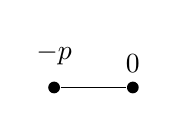
\begin{tikzpicture}[every node/.style={circle,fill=black,minimum width=1.5pt,inner sep=1.5pt}]
            \node[label={$-p$}] (A) at (0,0) {};
            \node[label={$0$}] (B) at (1,0) {};
            \draw (A) -- (B);
        \end{tikzpicture}
        \implies
        \begin{aligned}
            a_0 &= -1 & r_0 &= p \\
            a_1 &= 1 & r_1 &= 0
        \end{aligned}
    \end{equation*}
    $\mathbb{T}^1$ acts on $\mathbb{C}^2$ by $\lambda \cdot (z_1, z_2) = (\lambda z_1, \lambda z_2)$. $\pi=(-1,1)$ and $\iota=(1,1)^T$.
    The moment map $\iota^* \circ \mu : \mathbb{C}^2 \to (\mathfrak{t}^1)^*$ is given by
    \begin{equation*}
        \iota^*(\mu(z_1, z_2)) = \iota^*(-\pi|z_1|^2+p, -\pi|z_2|^2) = -\pi(|z_1|^2+|z_2|^2) + p.
    \end{equation*}
    Thus, $Z = (\iota^* \circ \mu)^{-1}(0) = \{ z \in \mathbb{C}^2 \mid |z|^2 = p/\pi \}$. Thinking $Z$ as $\mathbb{C}^2 / \mathbb{R}_{>0}$, $Z/\mathbb{T}^1 \cong \mathbb{P}^1$.

    For $\mathbb{P}^n$, consider the polytope
    \begin{equation*}
        \mathrm{conv}(\{ 0, e_1, \dots, e_n \})
        \implies
        \begin{aligned}
            a_0 &= (-1, \dots, -1) & r_0 &= p \in \mathbb{Z}_{>0} \\
            a_i &= e_i & r_i &= 0 \quad \forall 1 \leq i \leq n
        \end{aligned}
    \end{equation*}
    $\iota=(1,\dots ,1)^T$.
    Similarly, $\iota^* \circ \mu : \mathbb{C}^3 \to (\mathfrak{t}^1)^*$ is given by
    $\iota^*(\mu(z_0, \dots, z_n)) = -\pi(|z_0|^2+\cdots+|z_n|^2) + p$.
    $Z = (\iota^* \circ \mu)^{-1}(0) = \{ z \in \mathbb{C}^{n+1} \mid |z|^2 = p/\pi \}=\mathbb{C}^{n+1} / \mathbb{R}_{>0}/\mathbb{T}^1 \cong \mathbb{P}^n$.
\end{example}
\section{Hypertoric Varieties}
Hypertoric varieties is defined similar to the symplectic reduction construction for toric varieties $\mathbb{C}^n\GIT T_\mathbb{R}^k$. However, the fundamental building block changed to complex torus $T=\mathbb{C}^*$ acting on $T^*\mathbb{C}$ instead of $T_\mathbb{R}$ acting on $\mathbb{C}$; we use hyperplane arrangement instead of polytope.
\begin{example}[exp:]{$(\mathbb{C^*})^n\acton T^*\mathbb{C}^n$}
  The $T$-action on $T^*\mathbb{C}^n$ is given by $(t_iz_i,t^{-1}w_i)_{i=1}^{n}$. Let $X_i\in \mathfrak{t}^n$,
  \begin{alignat*}{1}
    (\ind{X_i})_z&=\frac{d}{dt}[e^{t_i}z_i,e^{-t_i}w_i]_{t=0}=(z_i\frac{\partial }{\partial z_i},-w_i\frac{\partial }{\partial w_i}),\\
    \iota_{\ind{X_i}}\omega&= (\sum_{}^{}dz_i\wedge dw_i)(z_i\partial/\partial z_i - w_i\partial/\partial w_i)=\sum z_idw_i + w_idz_i
  \end{alignat*}
  Hence $\mu(z_1,w_1,\dots ,z_n,w_n)=\sum_{}^{}z_iw_i$ is a choice of moment map.
\end{example}

Given a short exact sequence of complex tori
\begin{equation*}
    \begin{tikzcd}
        1 \arrow[r] & G \arrow[r, "\iota"] & D \arrow[r, "\pi"] & T \arrow[r] & 1
    \end{tikzcd}
\end{equation*}
with $ D \cong (\mathbb{C}^\times)^n $, we consider
\begin{enumerate}
    \item the $G$-action on $T^*\mathbb{C}^n$ by $ g \cdot (z, w) = (\iota(g)_iz_i, \iota(g)_i^{-1}w_i)_{i=1}^n $, and
    \item the moment map $ \mu : T^*\mathbb{C}^n \to \mathfrak{g}^* $ for the $G$-action given by $ (z, w) \mapsto \iota^*((z_iw_i)_{i=1}^n) $.
\end{enumerate}
Together with a character $ \chi : G \to \mathbb{C}^\times $ and $ \lambda \in \mathfrak{g}^* $, we define the hypertoric variety associated with these data to be the GIT quotient
\begin{equation*}
    \mathcal{M}_{\chi, \lambda} = T^*\mathbb{C}^n \HQ[\chi, \lambda] G = \mu^{-1}(\lambda) \GIT[\chi] G.
\end{equation*}
There is a remaining $T$-action on the quotient with a moment map $ \nu : \mathcal{M}_{\chi, \lambda} \to \mathfrak{t}^* $. We will always set $\lambda=0$. In this case, the above data can be assembled into a hyperplane arrangement with $n$ hyperplanes in the affine subspace $ (\iota_{\mathbb{R}}^*)^{-1}(\chi) = \{ x \in \mathfrak{d}_{\mathbb{R}}^* \mid \iota_{\Gamma}^*(x) = \chi \} $ of $\mathfrak{d}_{\mathbb{R}}^*$, where the $i$-th hyperplane is the intersection of $(\iota_{\mathbb{R}}^*)^{-1}(\chi)$ with the $i$-th coordinate hyperplane in $\mathfrak{d}_{\mathbb{R}}^*$. Conventionally, one choose a lift $\theta$ of $\chi$ along $\iota_\mathbb{R}^*$, allowing us to identify the affine subspace $(\iota_{\mathbb{R}}^*)^{-1}(\chi)$ with $\mathfrak{t}_\mathbb{R}^*$. This gives a hyperplane arrangement
\begin{equation*}
    \mathcal{A}_\chi = \{ H_i = \{ x \in \mathfrak{t}_{\mathbb{R}}^* \mid \pi^*(x)_i = \theta_i \} \}_{i=1}^n.
\end{equation*}
Different choices of lifts give the same hyperplane arrangement up to translations.
\section{Combinatorics of Graphs}

\subsection{GIT}
\subsection{Stability Condition}
For both $\theta$ and $\lambda$
\section{GKM Graph of Hypertoric}
\subsection{Fix Points}
\subsection{Connecting P1}
How $\theta$ effects the splitting of $S^+$
\subsection{Matroid Polytope}
\subsection{Equivariant Cohomology of Hypertoric}
\section{Line Bundles on Hypertoric}
\section{Steinberg Correspondences}
\subsection{Primitive Coroots and Hyperplane}
\subsection{Steinberg Varieties}

\section{Comparing Stability Condition with Quiver Varieties}

\appendix


%\bibliographystyle{alpha}
%\bibliography{ref}

\end{document}
